\documentclass[letterpaper,12pt]{article}
\usepackage{tabularx} % extra features for tabular environment
\usepackage{amsmath}  % improve math presentation
\usepackage{float}
\usepackage{pdfpages}

\usepackage{multicol}
\usepackage{graphicx} % takes care of graphic including machinery
\graphicspath{ {./figures/} }
%\usepackage[margin=1in,letterpaper]{geometry} % decreases margins
%\usepackage{cite} % takes care of citations
\usepackage[final]{hyperref} % adds hyper links inside the generated pdf file
\hypersetup{
	colorlinks=true,       % false: boxed links; true: colored links
	linkcolor=blue,        % color of internal links
	citecolor=blue,        % color of links to bibliography
	filecolor=magenta,     % color of file links
	urlcolor =blue         
}
\usepackage[margin = 1in,headsep=0.5cm,headheight=2cm,letterpaper]{geometry} 

\usepackage{fancyhdr}
\pagestyle{fancy}
\lhead{Student 1 : Ahmet Akman 2442366 \\ Student 2: Yusuf Toprak Yıldıran 2444149 \\ Assistant: Onur Selim Kılıç}
\rhead{Date: \today \\ Group: Wednesday Morning - 5} 
%\cfoot{center of the footer!}
\renewcommand{\headrulewidth}{0.1pt}



\begin{document}
\thispagestyle{empty}

\title{Spring 2022 EE214 Experiment 4  \protect\\ Impedance Measurement and Complex Power}
\author{Ahmet Akman 2442366 \protect\\ Yusuf Toprak Yıldıran 2444149 \protect\\ Assistant: Onur Selim Kılıç}
\date{\today}
\maketitle
\tableofcontents
%\begin{abstract}
%abstract
%\end{abstract}
\section{Introduction}
In this experiment, RMS values of voltages and currents will be measured, then the phase difference between current and voltage will be calculated, and complex power and power factor will be measured beside the apparent power S, the real power, and the reactive power with the efficiency of the system. Capacitance is aimed to be calculated using voltage and current RMS values. Afterward, two different modes of DSO will be used and explained to calculate impedance Z for different frequencies.

\section{Experimental Results and Discussion}
The results of the experiment are discussed in the following steps.
%
\subsection{Step 1}

In this part, circuit in Figure 1 is set with \(R_{line}= 100\Omega\) and \(Z_{load}= 560\Omega + j0.1w\) and inductor \(L= 0.1H\).

\begin{figure}[H]
    \centering
    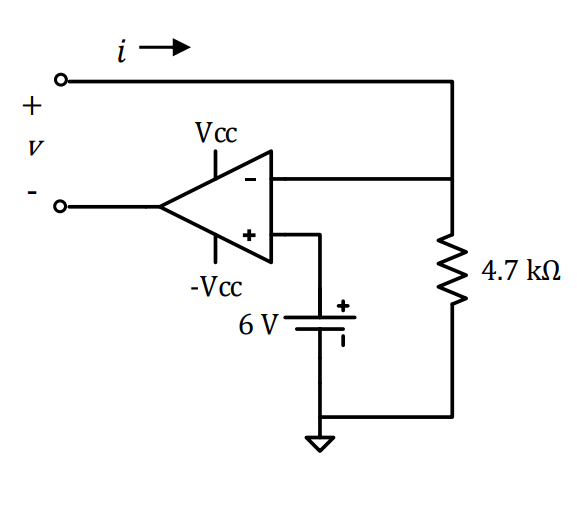
\includegraphics[width = 0.75\textwidth]{1SCH.png}
    \caption{Circuit schematic for the step 1}
\end{figure} 

For the parts below (a-b-c), magnitude of the voltage source is adjusted such that \(V_{load}(t)\) always equals to \(5sin(2000\pi t)\) V. 

\subsubsection{a.}
For this part, RMS values of \(V_{in}\), \(V_{line}\), \(V_{load}\), \(i_{load}\) and phase difference between \(V_{load}\) and \(i_{load}\) are measured and recorded in Table 1. RMS value of voltages is obtained by using the RMS measurement tool of DSO, and RMS current is obtained by measuring the voltage across \(100\Omega\) resistor. To calculate phase difference, the difference between peak values of the signals is measured in \(\mu s\), and proportionality with the 1/frequency value is found.

\vspace{2mm}
The | S |  (apparent power) parameter is found basically multiplying the RMS values of current and the voltage. Then to be able to find the resistive and reactive parts of the power, the power triangle is used. Using the phase difference $P_{Load}$ and $Q_{Load}$ parameters are obtained using $P_{load} = S\times cos(\phi)$ and $Q_{load} = S\times sin(\phi)$ identities respectively. Since the power line is assumed to be totally resistive, $P_{line}$ values are found by basically multiplying current with the voltage of the line. To find the $P{in}$ supplied by the source, it is assumed that there is no reactive source other than the load, so the phase angle of the load and the input is the same. So the power absorbed by load and line is added, and $P_{in}$ is obtained. The results are presented in Table 2.

\vspace{2mm}
Finally, the power factors are found from the cosine of the phase angles. The sign of the phase angle determines that the current is lagging (positive) or leading (negative). The efficiency is calculated from Table 2 by the fraction of $P{load}$ and $P_{in}$. The results are presented in Table 3.
\subsubsection{b.}
In this part, the 100nF capacitor is connected parallel with the load, and the exact measurements and calculations with part a. are made. Then, the results are recorded in Table 1 and Table 2.   
\subsubsection{c.}
For this part, the one \(\mu F\) capacitor is replaced with the 100nF capacitor in part a., and the same calculations and necessary measurements are made for this part as well.
\subsubsection{d.}
All the results of the measurements and calculations are given in this section as tabulated in Tables 1, 2, and 3.
\begin{table}[H]
    \begin{center}
        \caption{Power Measurements}
        \vspace{2mm}
        \begin{tabular}{||c | c | c | c | c | c | c ||} 
            \hline
            Part & \(V_{in}\)\newline (Vrms) & \(V_{line}\)\newline (Vrms) & \(V_{Load}\) \newline (Vrms) &\(i_{Load}\)\newline (mArms) & \(\phi_{Load}\) \newline(degree)& \(\phi_{in}\)\newline(degree) \\ [0.5ex] 
            \hline\hline
            a. & 3.7 & 0.4   & 3.4 & 4& 65  & 1.07 \\ 
            \hline
            b. &3.7 &0.3  &3.41 &  3 & 40& 0.57    \\
            \hline
            c. &4 &1.6  &3.4 &16 &-74 & 4.53  \\ [1ex] 
            \hline
        \end{tabular}
\end{center}
\end{table}


\begin{table}[H]
    \begin{center}
        \caption{Power Calcuations}
        \vspace{2mm}
        \begin{tabular}{||c | c | c | c | c | c ||} 
            \hline
            Part & \(P_{in}\)\newline (mW) & \(P_{line}\)\newline (mW) & \(P_{Load}\) \newline (mW) &\(Q_{Load}\)\newline (mVAR) & \(|S|_{Load}\)\newline(mVA)   \\ [0.5ex] 
            \hline\hline
            a. &7.34 & 1.6 & 5.74 & 12.32 & 13.6   \\ 
            \hline
            b. &8.73 & 0.9 & 7.83 & 6.58 &  10.23   \\
            \hline
            c. & 40.59 & 25.6 & 14.99 & 52.29  & 54.4   \\ [1ex] 
            \hline
        \end{tabular}
\end{center}
\end{table}




\begin{table}[H]
  \begin{center}
    \caption{Load Parameters}
    \vspace{2mm}
 \begin{tabular}{||lll|lll|lll||}
    \hline
    \multicolumn{3}{|l|}{Part a. (Load)}                            & \multicolumn{3}{l|}{Part b. Load}                            & \multicolumn{3}{l|}{Part c. Load}                            \\ \hline
    \multicolumn{1}{|l|}{pf} & \multicolumn{1}{l|}{lead/lag} & eff \(\%\) & \multicolumn{1}{l|}{pf} & \multicolumn{1}{l|}{lead/lag} &eff \(\%\)  & \multicolumn{1}{l|}{pf} & \multicolumn{1}{l|}{lead/lag} &eff \(\%\)  \\ \hline
    \multicolumn{1}{|l|}{0.42} & \multicolumn{1}{l|}{lagging} & 78 & \multicolumn{1}{l|}{0.76} & \multicolumn{1}{l|}{lagging} & 90 & \multicolumn{1}{l|}{0.28} & \multicolumn{1}{l|}{leading} & 37 \\ \hline
    \end{tabular}.
\end{center}

\end{table}

It can be concluded for this step that power factor correction might help the real power to be dominant in the overall power supplied so that the efficiency might be increased. However, power factor correction needs to be done meticulously such that an overcompensated phase angle may lead to worse efficiency, as happened in part c.


\subsection{Step 2}

In this step, the circuit in figure 2 is set by adjusting signal generator output to a sine wave with 500 Hz frequency and 6 Volt peak to peak voltage value using one \(\mu F\) capacitor and one \(k\Omega \) resistor to obtain current. Then, the RMS value of the voltage V across the capacitor is measured as 1.23 V, and the RMS value of the current passing through the capacitor is measured as 3.70 mA. Afterward, by doing the following calculations, capacitance C1 is calculated:

\[\frac{V_{rms}}{i_{rms}} = |Z| = \frac{(-j)^2}{w^2C^2}\]
where Z is the impedance and w = \(2\pi (500 Hz)\).  
\[C1 = \frac{i_{rms}}{V_{rms}\omega}  =  \frac{3.79 mA}{1.23 V . 1000\pi} \approx 0.98x10^{-6} = 0.98 \mu F\]

Then by adjusting LC meter to proper scale, nominal capacitance of the capacitor is measured as 1.03 \(\mu F\)
\begin{figure}[H]
    \centering
    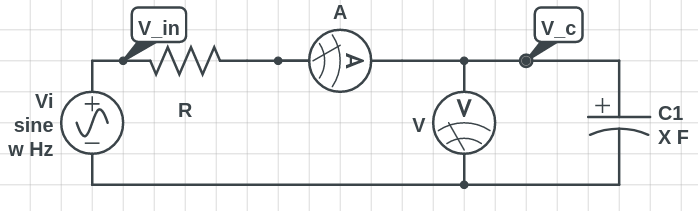
\includegraphics[width = 0.75\textwidth]{2SCH.png}
    \caption{Circuit schematic for the step 2}
\end{figure} 
    
\subsection{Step 3}

In this step, the circuit in figure 4 is set with 1.5 kHz and 3 kHz frequency sine wave, respectively, and 0.1 \(\mu F\) capacitor and 1k\(\Omega \) resistor and 0.1 H inductor are used, then by using two different methods, impedance Z in Figure 3 is measured. To be able to measure , A and B terminals of the load is connected to the A and B terminals of the circuit given in Figure 4.
\begin{figure}[H]
    \centering
    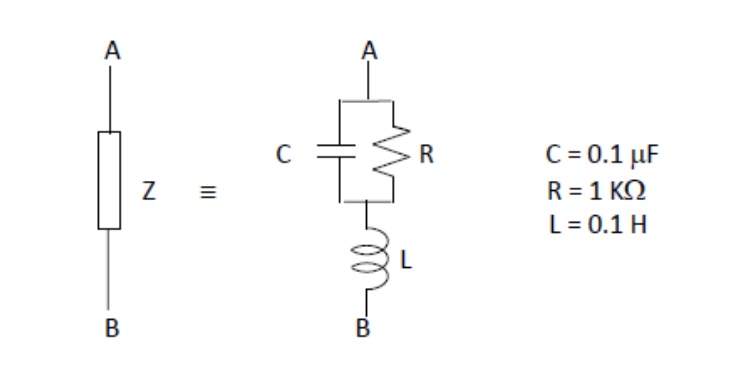
\includegraphics[width = 0.75\textwidth]{3SCH.png}
    \caption{Circuit schematic for the step 3}
\end{figure} 

\begin{figure}[H]
    \centering
    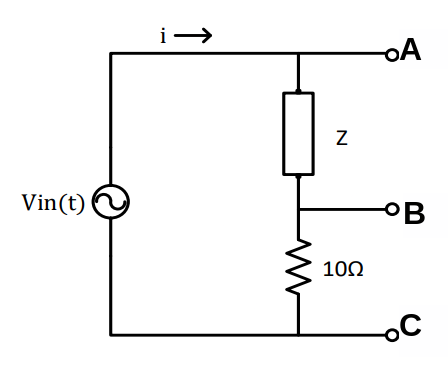
\includegraphics[width = 0.75\textwidth]{3_1SCH.png}
    \caption{Outside circuit schematic for the step 3}
\end{figure} 

\subsubsection{First Method}
In the first method, the probes of the oscilloscope are connected to the A, B, and C terminals as follows. Terminal A is connected to the CH1, and Terminal C is connected to the CH2. Terminal B is connected to the common ground. Then the adjustment is made that CH2 is inverted in the oscilloscope. So, the CH2 corresponds to the current flowing through the circuit. \\ By ignoring the resistance of the 10 Ohm resistor, the phase angle is measured in XY mode. 
\begin{figure}[H]
    \centering
    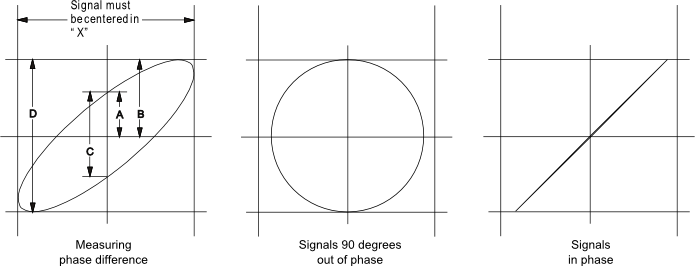
\includegraphics[width = 0.75\textwidth]{4PHASE.jpeg}
    \caption{XY mode phase difference guide}
\end{figure} 
The sketches given in Figure 5 is taken from the manufacturer of the DSO's used in laboratory (\href{https://edadocs.software.keysight.com/kkbopen/xy-display-mode-example-589308984.html}{Source}) . The phase difference is found by the following equation: 
\[ 
    \phi = \arcsin(\frac{C}{D}) = \arcsin(\frac{A}{B})
    \]

\subsubsection{Second Method}
In the second method, the setup described in the first method is conserved, but instead of XY mode, the time mode of the DSO is used. Here, simply the measure feature of the DSO is used, and the same results are obtained. The results of the measurements made in Step 3 are given in Table 4 and Table 5.

\begin{table}[H]
    \begin{center}
        \caption{Power Measurements in Step 3 (1.5kHz)}
        \vspace{2mm}
        \begin{tabular}{||c | c | c | c ||} 
            \hline
            CH1 (Voltage) & CH2 (mAmps) & Phase Angle (degrees) & Impedance (Ohms)   \\ [0.5ex] 
            \hline\hline
            4 & 5  & 40    & 800  \\ 
            \hline
        \end{tabular}
\end{center}
\end{table}

\begin{table}[H]
    \begin{center}
        \caption{Power Measurements in Step 3 (3kHz)}
        \vspace{2mm}
        \begin{tabular}{||c | c | c | c ||} 
            \hline
            CH1 (Voltage) & CH2 (mAmps) & Phase Angle (degrees) & Impedance (Ohms)   \\ [0.5ex] 
            \hline\hline
            4.2 & 2.7  & 80    & 1555   \\ 
            \hline
        \end{tabular}
\end{center}
\end{table}

\section{Conclusion}
In this experiment, RMS values of voltages and currents are measured. Phase differences between current and voltage are calculated, and complex power and power factor are measured beside the apparent power S, the real power, and the reactive power with the efficiency of the system. Capacitance is calculated using voltage and current RMS values. Lastly, two different modes of DSO are used and explained to calculate impedance Z for two different frequencies.


\section*{Appendix A}
\begin{itemize}
    \item PreLab Preparation 3 hours
    \item Experimental Work 2  hours
    \item Report Writing 8 hours
\end{itemize}
\section*{Appendix B}
In this experiment, since the values the students obtained in the lab is quite close to the data provided by the lab assistants, it is preffered to use the data obtained by the students.

\end{document}

%%%%%%%%%%%%%%%%%%%%%%   EXAMPLE TABLE   %%%%%%%%%%%%%%%%%%%%%%%%%%%%%%%%
\begin{table}[H]
\begin{center}
    \caption{Resistance reading by color code convention.}
    \vspace{2mm}
    \begin{tabular}{||c | c | c||} 
        \hline
        Color Order & Value & Tolerance \\ [0.5ex] 
        \hline\hline
        Brown / Black / Red / Gold & 1k\( \Omega \) & \( \% \) 5  \\ 
        \hline
        Yellow / Violet / Red / Gold & 4.7k\( \Omega \) & \( \% \) 5   \\
        \hline
        Brown / Grey / Orange / Gold & 18k\( \Omega \) & \( \% \) 5  \\ [1ex] 
        \hline
    \end{tabular}
\end{center}
\end{table}


%%%%%%%%%%%%%%%%%%%%%%   EXAMPLE IMAGE   %%%%%%%%%%%%%%%%%%%%%%%%%%%%%%%%
\begin{figure}[H]
\centering
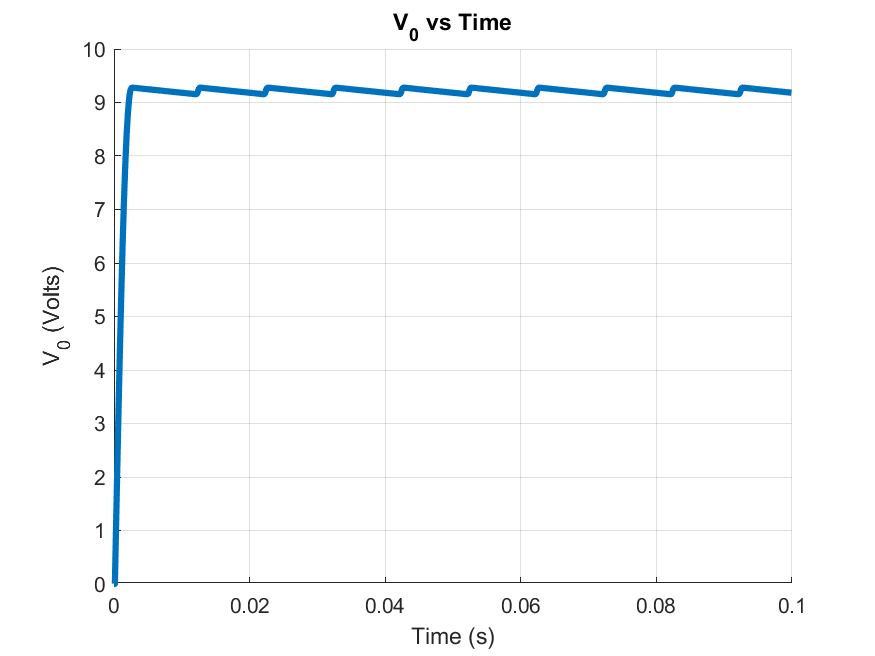
\includegraphics[width = 0.75\textwidth]{5.png}
\caption{Circuit schematic for the step 5}
\end{figure} 

%%%%%%%%%%%%%%%%%%%%%%   EXAMPLE IMAGE FROM PDF   %%%%%%%%%%%%%%%%%%%%%%%%%%%%%%%%
\begin{figure}[H] \centering{
	\includegraphics[scale=0.25]{2a_plot.pdf}}
	\caption{Experiment 2}
\end{figure}
%%%%%%%%%%%%%%%% Deneme Push